\documentclass[xcolor=dvipsnames]{beamer} 
\usepackage[spanish,mexico]{babel}
\usepackage[latin1]{inputenc}
\usepackage{amsmath}
\usepackage{amsfonts}
\usepackage{amssymb}
\usepackage{subcaption}
\usepackage{graphicx}
\usepackage{hyperref}
\usepackage{movie15}
\usepackage[style=verbose,backend=biber,citestyle=authoryear]{biblatex}
\addbibresource{expo.bib}

%\usecolortheme[named=Green]{structure} 
\usetheme{Frankfurt}
%\useoutertheme{shadow} % Alternatively: miniframes, infolines, split
\setbeamercolor{structure}{bg=black, fg=black}
\useinnertheme{circles}
 
\author{M. en F. Carlos Manuel Rodr�guez Mart�nez \\ Advisor: Dr. Alejandro Ra�l Hern�ndez Montoya}
\institute{Universidad Veracruzana}
\title{A multi-scale symmetry analysis of daily financial time series using uninterrupted trends returns}
\date{\today}

\makeatletter
\let\@@magyar@captionfix\relax
\makeatother

\begin{document}

\begin{frame}
\maketitle
\end{frame}

%-----------------------------------------------------------------------------
\begin{frame}
\section{Acknowledgments}
\textbf{Acknowledgments}
\begin{itemize}
	\item Dr. Alejandro Ra�l Hernandez Montoya. Universidad Veracruzana.
	\item Dr. Hector Conoronel Brizio. Universidad Veracruzana.
\end{itemize}
\end{frame}


%-----------------------------------------------------------------------------
\setbeamercolor{structure}{fg=blue!50!black!40!green}
\begin{frame}
\section{Introduction}
\textbf{Introduction}
\end{frame}

%-----------------------------------------------------------------------------
\begin{frame}{Publicly available information}
  Prices, volume, dividends, beta, etc.
  \begin{figure}
        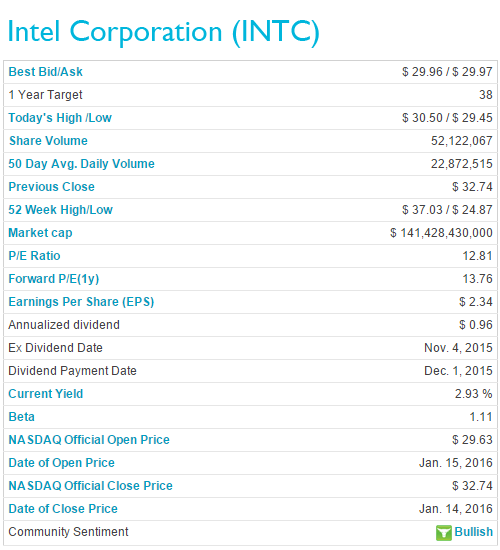
\includegraphics[scale=0.60]{img/NASDAQ_INTC}
  \end{figure}
\end{frame}

%-----------------------------------------------------------------------------
\begin{frame}{What is relevant to price}
  \begin{itemize}
  \item Interaction of many agents that perform buy/sell operations.
  \item Every agent has access to the same public information to make an informed decision on every operation. They are rational.
  \item The direct consequence is that current price already contains all the knowledge of future forecasts.
  \[
	E\left[P_{t+1}|P_0,\,P_1, \dots, P_t \right] = P_t.
  \]
  \begin{figure}
        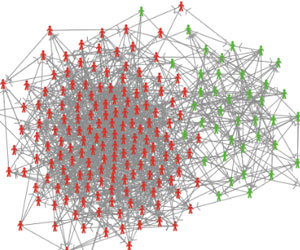
\includegraphics[scale=0.30]{img/agent}
  \end{figure}
  \end{itemize}
\end{frame}

%-----------------------------------------------------------------------------
\begin{frame}{Efficient market hypothesis (EMH)}
  \begin{itemize}
  \item Bachelier 1900 proposes that since in a voluntary stock exchange between two agents, each of them believes them to be the winning party. If the game is fair (Martingale) it must behave like a random walk. His work was not well received.
  \item \cite{Samuelson} proposes the efficient market hypothesis. If investors were able to incorporate future events in the current price, they would have done so, incorporating their knowledge in the current price.
  \item \cite{Fama1995} finds empirical evidence that markets behave like a random walk.
  \item The EMH requires agents to be rational.
  \end{itemize}
\end{frame}

%-----------------------------------------------------------------------------
\begin{frame}{An historical example}
  \begin{itemize}
  \item Challenger space shuttle. Four contractors involved: Lockheed, Martin Marietta, Morton Thiokol y Rockwell.
  \item After 5 months of investigation it was found that the misbehaving component came from Morton Thiokol.
  \item Markets declared their verdict right away.
  \begin{figure}
        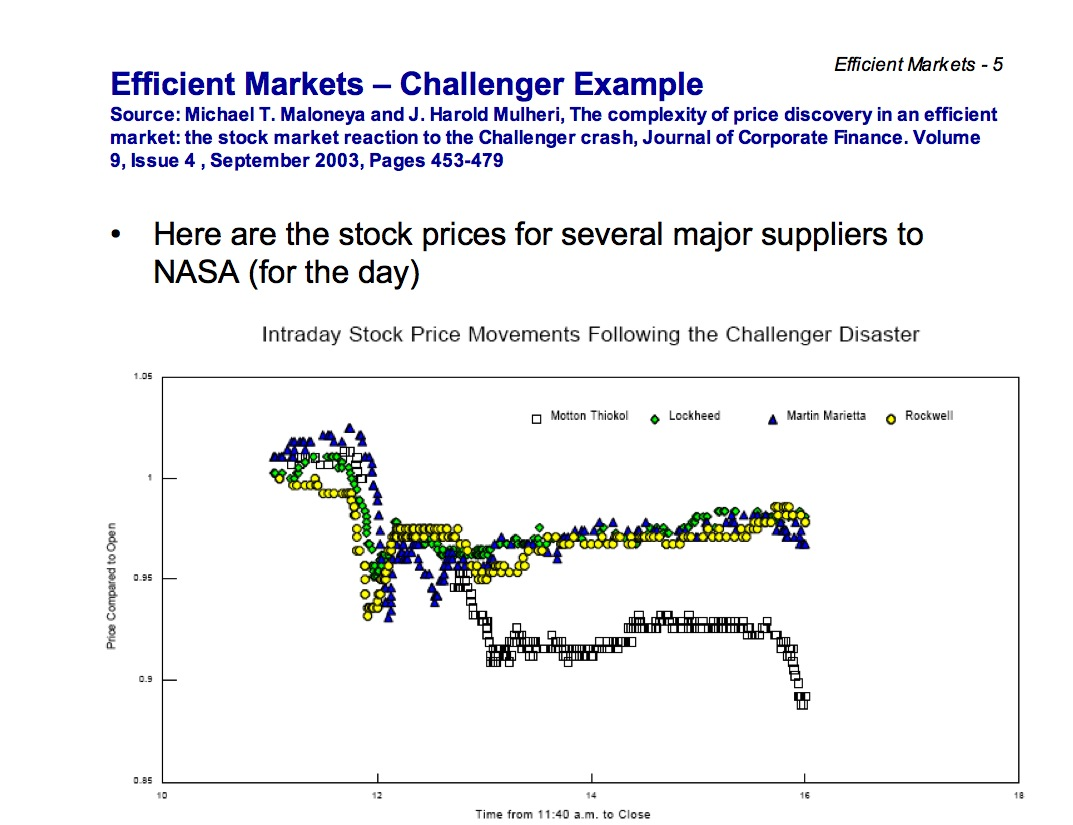
\includegraphics[scale=0.16]{img/challenger}
  \end{figure}
  \end{itemize}
\end{frame}


%-----------------------------------------------------------------------------
\begin{frame}{If I can't win there is no point}
  \begin{itemize}
  \item \cite{Markowitz1952} optimal portfolio theory tell us that we can construct a portfolio such that the relation between expected return and risk is optimal.
  \begin{figure}
        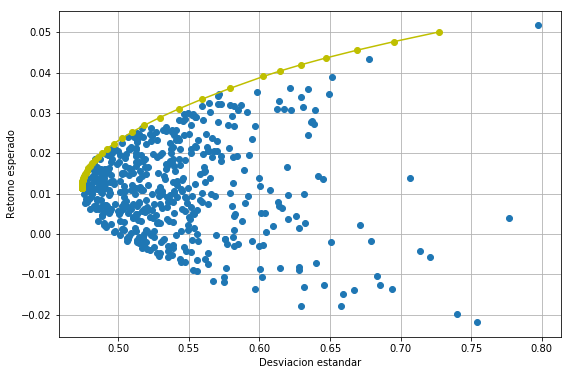
\includegraphics[scale=0.30]{img/portafolio}
  \end{figure}
  \item Useful for long term investment.
  \item EMH implies the reliability of predictive markets.
  \end{itemize}
\end{frame}

%-----------------------------------------------------------------------------
\begin{frame}{There are winners however...}
  \begin{itemize}
  \item The existence of agents that can reliably generate profits like Warren Buffet, Peter Lynch and George Soros, implies the possibility that some agents can sometimes predict better than others future outcomes.
  \item Humans have cognitive biases that systematically makes us averse to lose and have high hopes of winning. We are not always rational.
  \end{itemize}
\end{frame}

%-----------------------------------------------------------------------------
\begin{frame}{Motivation}
  How can we assess the efficiency of a market?
\end{frame}

%-----------------------------------------------------------------------------
\begin{frame}
\section{Background}
\textbf{Background}
\end{frame}

%-----------------------------------------------------------------------------
\setbeamercolor{structure}{fg=cyan!90!cyan}
\begin{frame}{Definitions}
  \begin{itemize}
    \item We define the logarithmic returns as
    \[
  		R(t,\Delta t) = \log P_{t+\Delta t} - \log P_t.
    \]
    \begin{figure}
        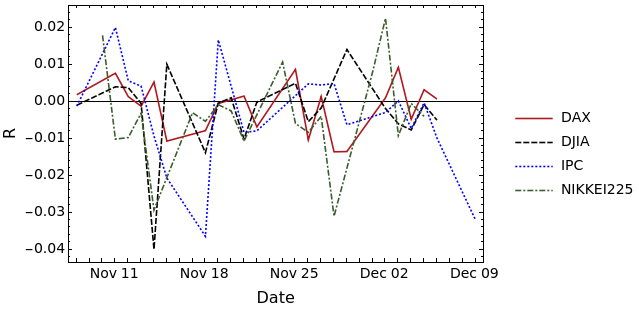
\includegraphics[scale=0.23]{img2/returns.png}
    \end{figure}
    \item We can express the efficient market hypothesis in terms of the returns
    \[
		E\left[R_{t+1}|R_0,\,R_1, \dots, R_t \right] = 0.
  	\]
  	\item From this definition of the returns emerge the \textit{stylized facts}, that are statistical properties common to the returns of most markets.
  \end{itemize}
\end{frame}

%-----------------------------------------------------------------------------
\setbeamercolor{structure}{fg=cyan!90!cyan}
\begin{frame}[allowframebreaks]
\frametitle{Stylized facts}
  \begin{itemize}
  \item Win / Loss assymetry. Symmetry is strongly related to the EMH.
  \begin{figure}
        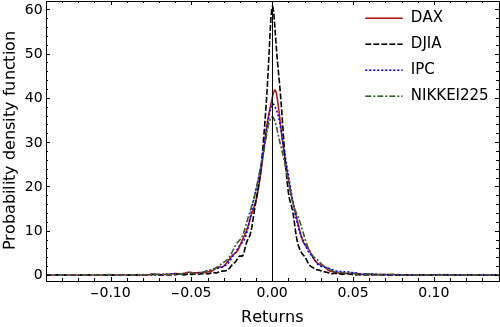
\includegraphics[scale=0.3]{img/Asim}
  \end{figure}
  \item No auto-correlation on the returns
  \begin{figure}
        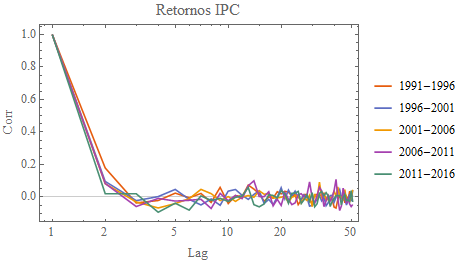
\includegraphics[scale=0.35]{img/Efficiency}
  \end{figure}
  \item Returns decay as a power law.
  \begin{figure}
        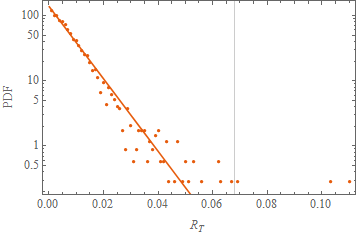
\includegraphics[scale=0.38]{img/RetSimplesLeyPot}
  \end{figure}
  \item Some events extremely rare (according to the power law) still happen sometimes. We identify these extreme events as the Dragon Kings described by Sornette. Usually these extreme values signal a big transition in the market like an economic crisis.
    \begin{figure}
        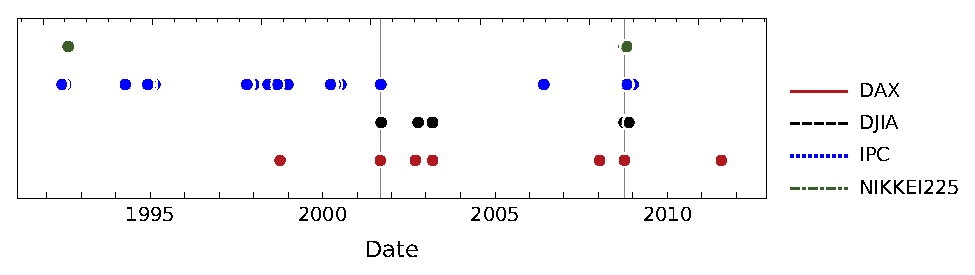
\includegraphics[scale=0.4]{img4/extreme_events}
  \end{figure}
  
  \item Volatility clustering
  \[
	C_2(\tau) = \operatorname{Corr}(R(t+\tau, \Delta t)^2,\, R(t, \Delta t)^2).
  \]
  That is, big changes tend to be followed by big changes of any sign, and small changes tend to be followed also by small changes of any sign.
  \begin{figure}[h!]
\begin{subfigure}{.5\textwidth}
	\centering
	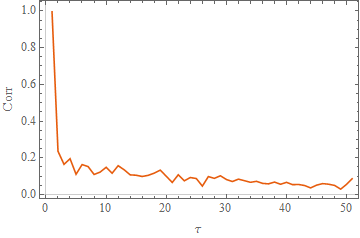
\includegraphics[scale=0.3]{img/Volatility}
\end{subfigure}%
\begin{subfigure}{.5\textwidth}
	\centering
	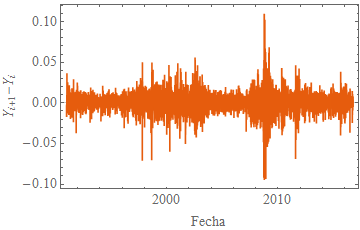
\includegraphics[scale=0.3]{img/RetST}
\end{subfigure}%
\end{figure}

  \end{itemize}
\end{frame}


%-----------------------------------------------------------------------------
\setbeamercolor{structure}{fg=cyan!20!blue}
\begin{frame}{H.F. Coronel-Brizio, et al. (2007) Assessing symmetry of financial returns series. Physica A 383.}
\section{A test for symmetry}
\textbf{A test for symmetry}
	\begin{itemize}
	\item Based on the $T_n$ statistic developed by Einmahl and McKeague.
	\item The null hypothesis is that there is a symmetry point around $c$, that is $H_0: F(c-x) = 1 - F(x-c)$, for every $x>0$ in the sample $X_1, \dots, X_n$. $F$ is a cumulative distribution function.
	\end{itemize}
\end{frame}

\begin{frame}{Einmahl, McKeague (2003) Empirical likelihood based hypothesis testing I}
	\begin{figure}
        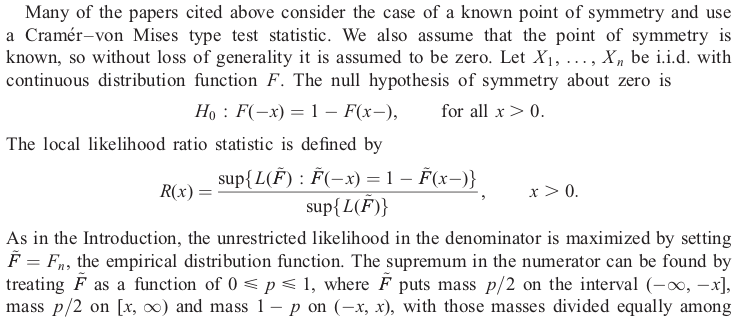
\includegraphics[scale=0.43]{img2/Hoja1.png}
    \end{figure}
\end{frame}

\begin{frame}{Einmahl, McKeague (2003) Empirical likelihood based hypothesis testing II}
	\begin{figure}
        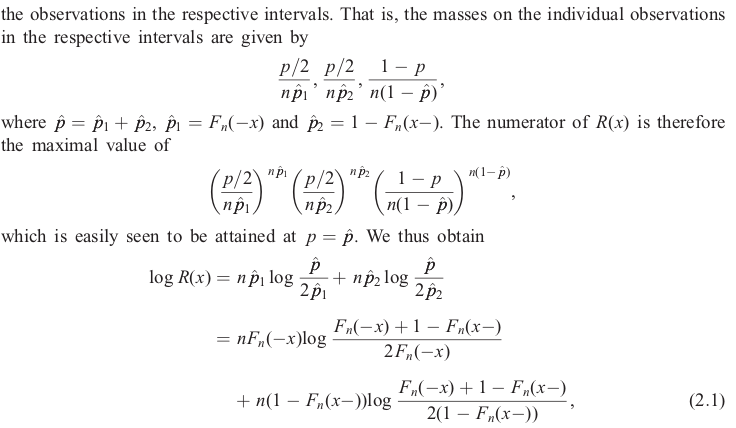
\includegraphics[scale=0.43]{img2/Hoja25.png}
    \end{figure}
\end{frame}

\begin{frame}{A quick visualization}
Simulation of 100 normally distributed numbers. The weight transformation is applied.
	\begin{figure}[h!]
		\begin{subfigure}{.5\textwidth}
			\centering
			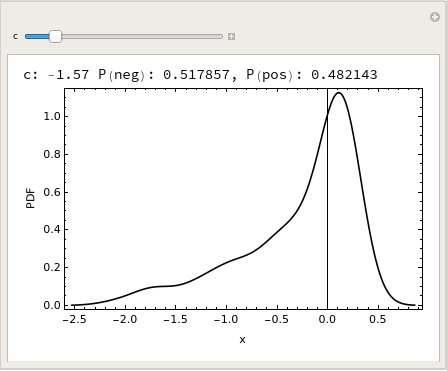
\includegraphics[scale=0.25]{img2/transform1}
		\end{subfigure}%
		\begin{subfigure}{.5\textwidth}
			\centering
			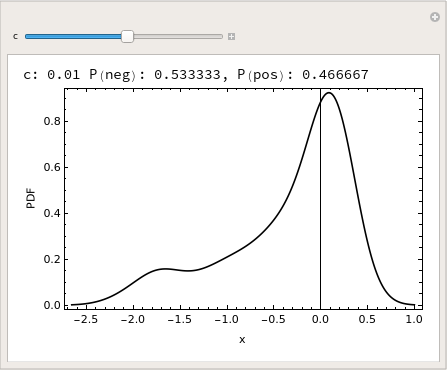
\includegraphics[scale=0.25]{img2/transform2}
		\end{subfigure}%
	\end{figure}
	\begin{figure}
        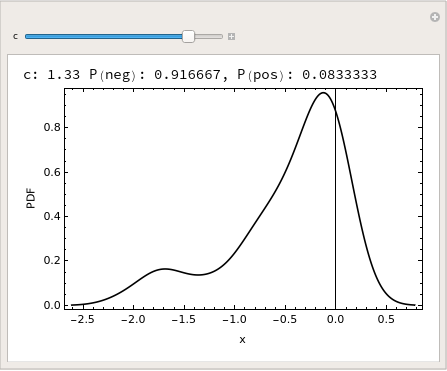
\includegraphics[scale=0.25]{img2/transform3}
    \end{figure}
\end{frame}

\begin{frame}{A quick visualization}
	\begin{figure}
        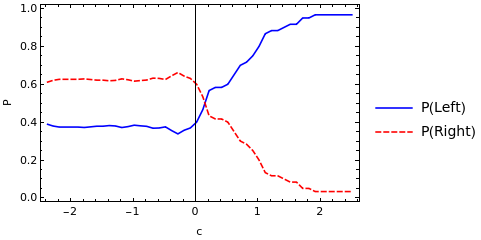
\includegraphics[scale=0.35]{img2/ps}
        \caption{Left and right cumulative distribution functions.}
    \end{figure}
    
\end{frame}

%-----------------------------------------------------------------------------
\begin{frame}{H.F. Coronel-Brizio, et al. (2007) Assessing symmetry of financial returns series. Physica A 383.}
	\begin{itemize}
	\item The statistic $T_n$ around a test point $c$ is
	\[
		T_n =  - \frac{2}{n} \sum_{i=1}^n \log R(|X_i|).
	\]
	where
	\begin{align*}
		\log R(x) &= n F_n (c-x) \log \frac{F_n(c-x)+1-F_n(x-c)}{2F_n(c-x)} \\
		&+ n(1-F_n(x-c)) \log \frac{F_n(c-x)+1-F_n(x-c)}{2(1-F_n(x-c))}.
	\end{align*}
	and $F_n$ is the cumulative empirical distribution function.
	\end{itemize}
\end{frame}

%-----------------------------------------------------------------------------
\begin{frame}{H.F. Coronel-Brizio, et al. (2007) Assessing symmetry of financial returns series. Physica A 383.}
	\begin{itemize}
	\item We can test for $c$ in an interval $[C_{min},C_{max}]$, for example
	  \begin{figure}
        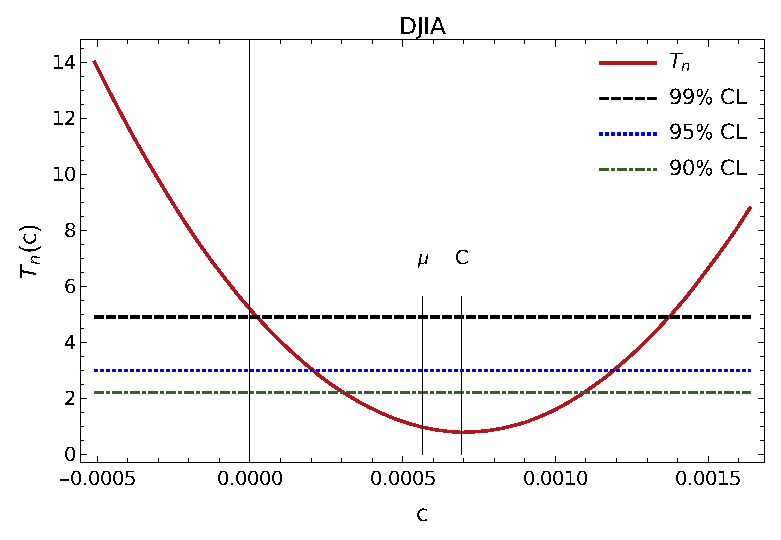
\includegraphics[scale=0.3]{img4/SymmetryPlots/simetria_TReturns_DJIA}
        \caption{$T_n$ symmetry test evaluated on the returns of the DJIA index.}
  \end{figure}
	\item We can affirm with 95 \% certainty that the distribution is symmetrical in a interval between 0.0002 and 0.001.
	\end{itemize}

\end{frame}



%-----------------------------------------------------------------------------
\begin{frame}{The problem of scale}
	\begin{itemize}
	\item The time lag in which the returns are defined are particularly relevant when measuring symmetry.
     \begin{figure}
        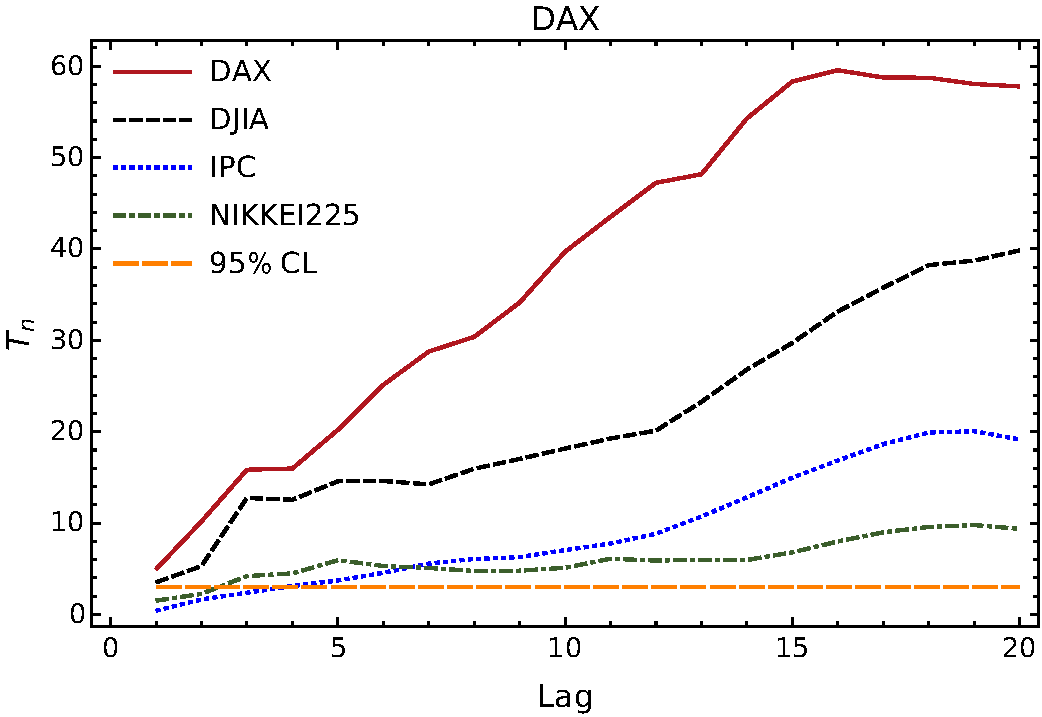
\includegraphics[scale=0.33]{img2/tns_lag.pdf}
        \caption{$T_n(0)$ with returns of different lags.}
     \end{figure}
     \item Artifacts are introduced with this methodology.
	\end{itemize}
\end{frame}

%-----------------------------------------------------------------------------
\begin{frame}{Definition of trend returns}
  \begin{itemize}
  \item Multiscale return definition. Given a financial time series $P_{1},\ldots,P_{n}$, we define an ``uninterrupted trend'' of duration  $k$, a succession of $k+1$ consecutive values of the given time series where each value is greater than the preceding one.
  \item We define their corresponding trend return as:
	\begin{equation}
		TRet_m^k := \log(P_{m+k}) - \log(P_{m})  
	\end{equation}
Where $m$ indexes the different trends and $k$ indicates the duration in days of $m$-Th trend.
  \begin{figure}
        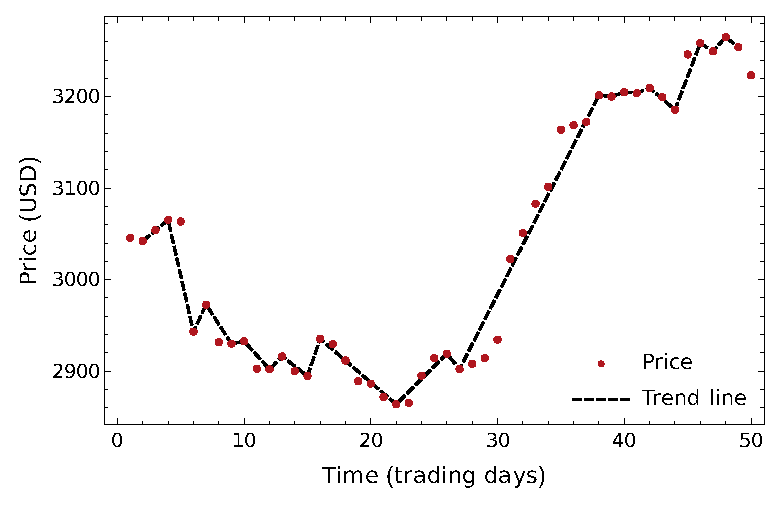
\includegraphics[scale=0.33]{img/TrendLines.eps}
  \end{figure}
  \end{itemize}
\end{frame}

%-----------------------------------------------------------------------------
\begin{frame}
\frametitle{Trend returns distribution}
	Analogously we can define the \textit{trend velocity returns} as the rate in which the trend returns change.
	\begin{equation}
		TVRet_m^k := \frac{\log(P_{m+k}) - \log(P_{m})}{k}  
	\end{equation}
  	  \begin{figure}[h!]
		\begin{subfigure}{.5\textwidth}
			\centering
			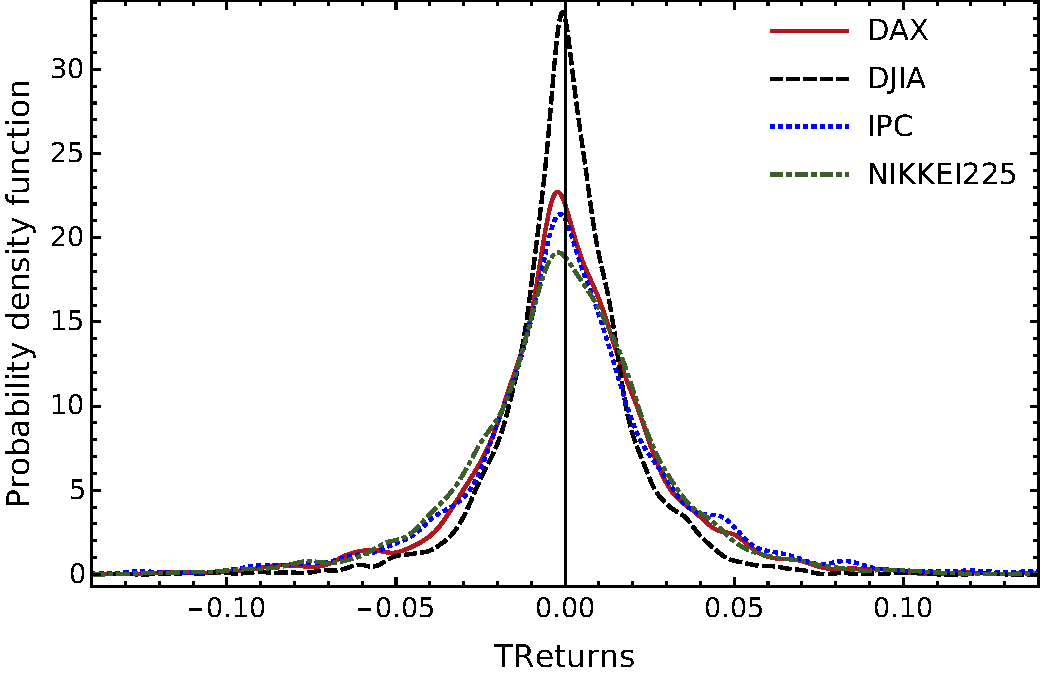
\includegraphics[scale=0.3]{img4/tret_dist}
		\end{subfigure}%
		\begin{subfigure}{.5\textwidth}
			\centering
			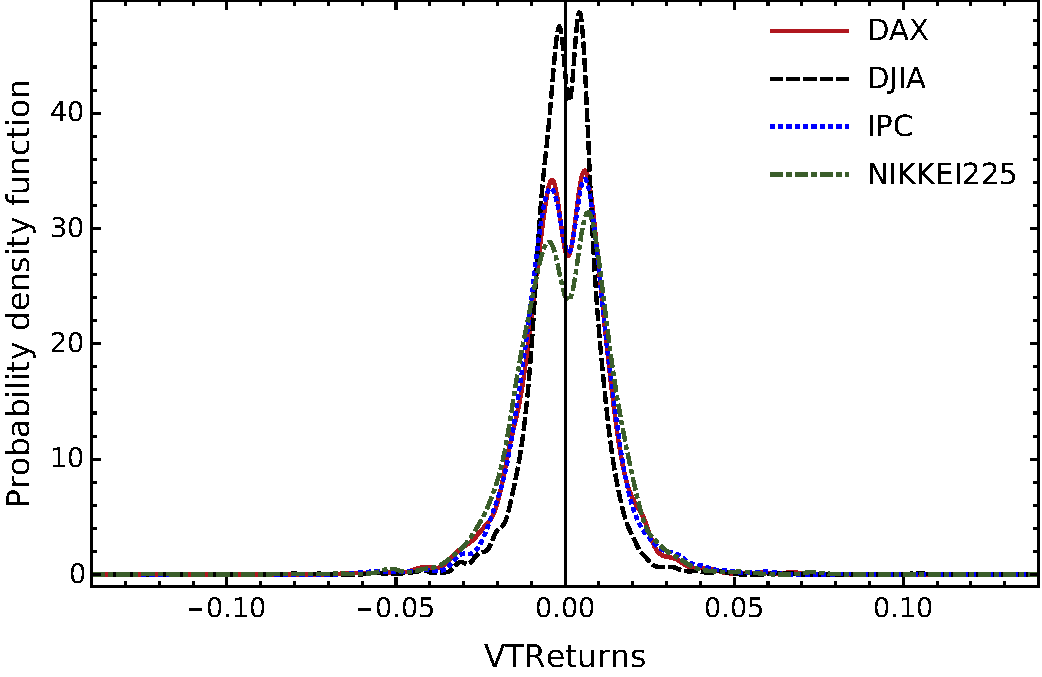
\includegraphics[scale=0.3]{img4/tvret_dist}
		\end{subfigure}%
	  \end{figure}
\end{frame}

%-----------------------------------------------------------------------------
\begin{frame}[allowframebreaks]
  \frametitle{This definition also comes with its stylized facts}
  \begin{itemize}
  \item Volatility clustering is present in trend returns $R_m^k$
  	  \begin{figure}[h!]
		\begin{subfigure}{.5\textwidth}
			\centering
			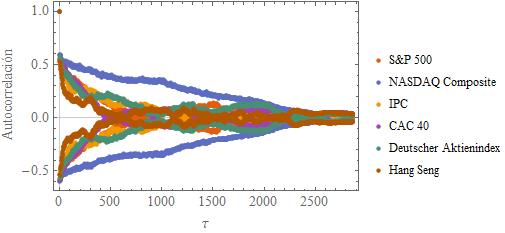
\includegraphics[scale=0.30]{img3/ACF_RT}
			\caption{Trend returns autocorrelation.}
		\end{subfigure}%
		\begin{subfigure}{.5\textwidth}
			\centering
			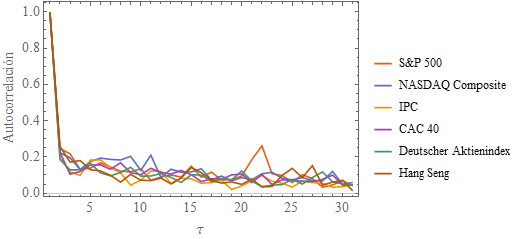
\includegraphics[scale=0.30]{img3/ACF_RT2}
			\caption{Quadratic trend returns autocorrelation.}
		\end{subfigure}%
	\end{figure}
	\item So trend returns still can be decomposed as
	\[
		R_T(t) = \sigma_R(t) \epsilon(t),
	\]
	where $\epsilon(t)$ is gaussian noise and $\sigma(t)$ the volatility.
  \end{itemize}

\textbf{H.F. Coronel-Brizio, A.R. Hernandez-Montoya (2005). On fitting the Pareto-Levy distribution to stock market index data: selecting a
suitable cut off value. Physica A 354 437-449.}
Describes a procedure to select the cutoff point where returns start behaving as a power law.
  \begin{figure}
        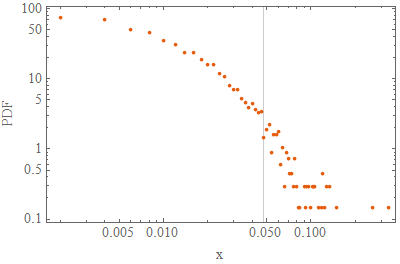
\includegraphics[scale=0.50]{img3/Neg1.png}
  \end{figure}
\end{frame}

%-----------------------------------------------------------------------------
\setbeamercolor{structure}{fg=red!50!black!50!red}
\begin{frame}
\section{Results}
\textbf{Results}
\end{frame}

%-----------------------------------------------------------------------------
\begin{frame}
\frametitle{Symmetry tests: Trend returns}
  	  \begin{figure}[h!]
		\begin{subfigure}{.5\textwidth}
			\centering
			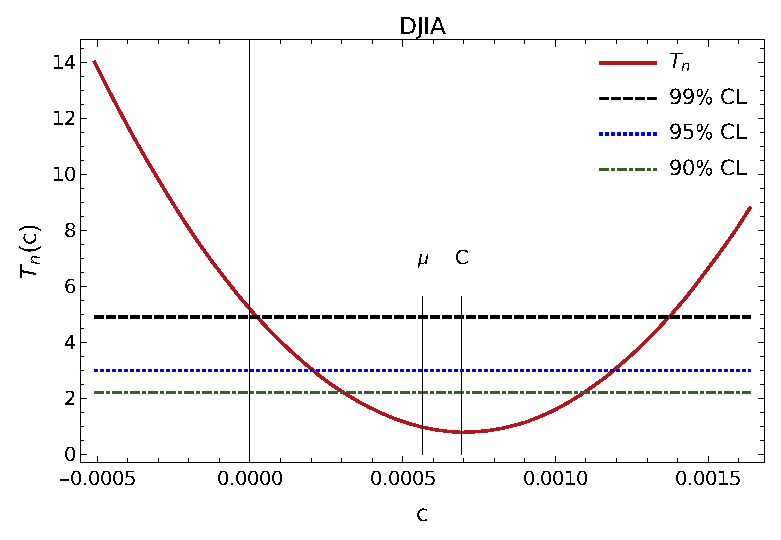
\includegraphics[scale=0.3]{img4/SymmetryPlots/simetria_TReturns_DJIA}
		\end{subfigure}%
		\begin{subfigure}{.5\textwidth}
			\centering
			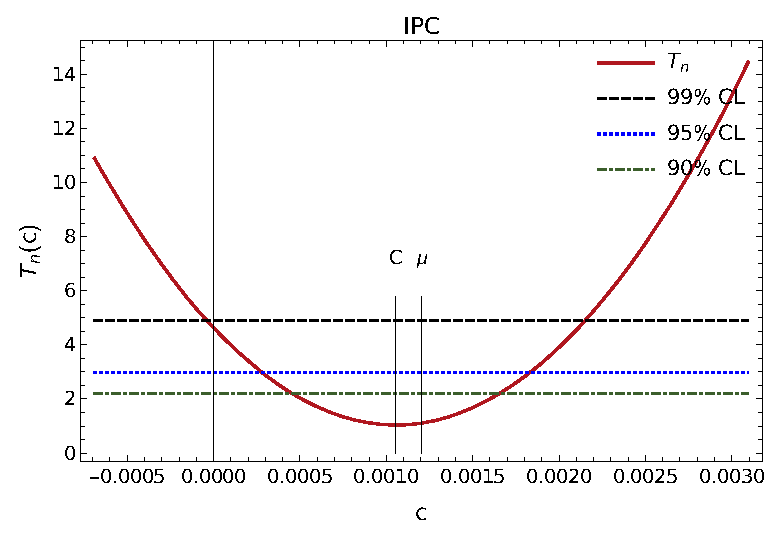
\includegraphics[scale=0.3]{img4/SymmetryPlots/simetria_TReturns_IPC}
		\end{subfigure}%
	\end{figure}
	  	  \begin{figure}[h!]
		\begin{subfigure}{.5\textwidth}
			\centering
			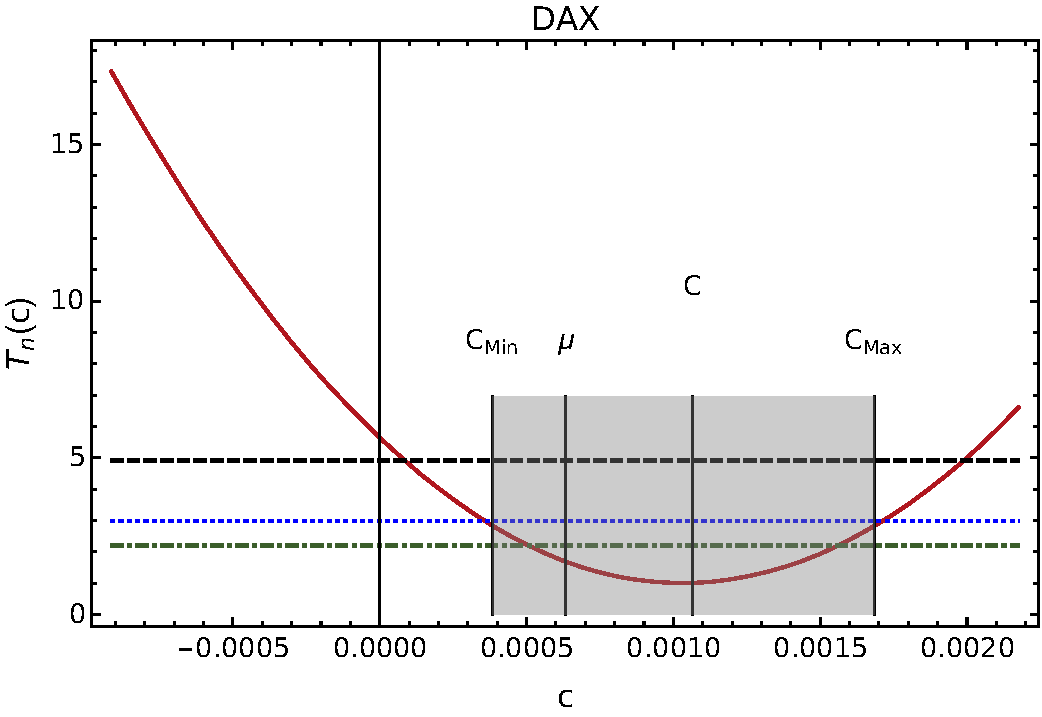
\includegraphics[scale=0.3]{img4/SymmetryPlots/simetria_TReturns_DAX}
		\end{subfigure}%
		\begin{subfigure}{.5\textwidth}
			\centering
			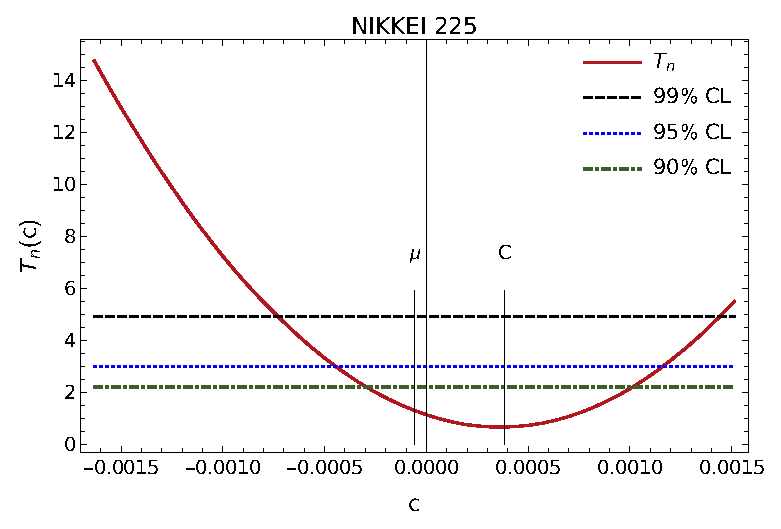
\includegraphics[scale=0.3]{img4/SymmetryPlots/simetria_TReturns_NIKKEI225}
		\end{subfigure}%
	\end{figure}
\end{frame}

%-----------------------------------------------------------------------------
\begin{frame}
\frametitle{Time evolution of the most plausible point of symmetry: Simple returns}
  	  \begin{figure}[h!]
		\begin{subfigure}{.5\textwidth}
			\centering
			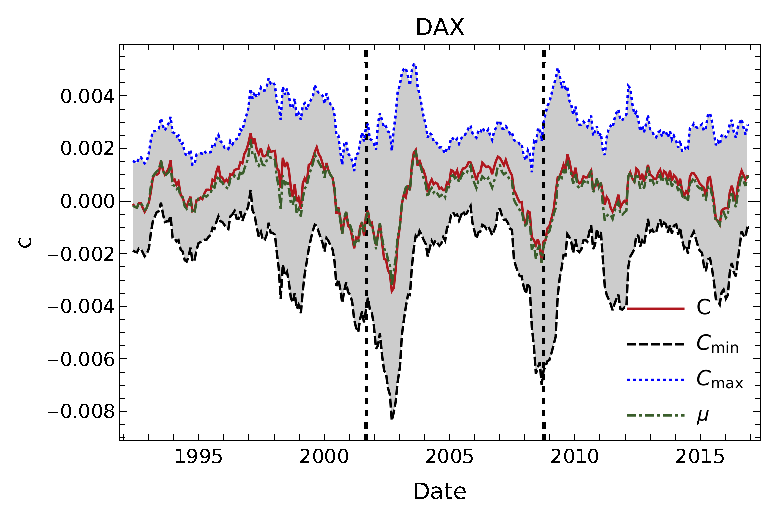
\includegraphics[scale=0.35]{img4/SimmReturns/Simetria_DAX_CL005}
		\end{subfigure}%
		\begin{subfigure}{.5\textwidth}
			\centering
			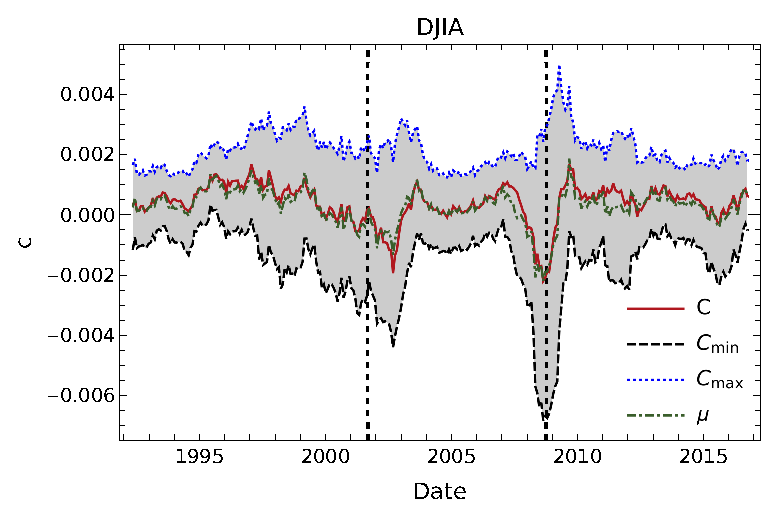
\includegraphics[scale=0.35]{img4/SimmReturns/Simetria_DJIA_CL005}
		\end{subfigure}%
	\end{figure}
	  	  \begin{figure}[h!]
		\begin{subfigure}{.5\textwidth}
			\centering
			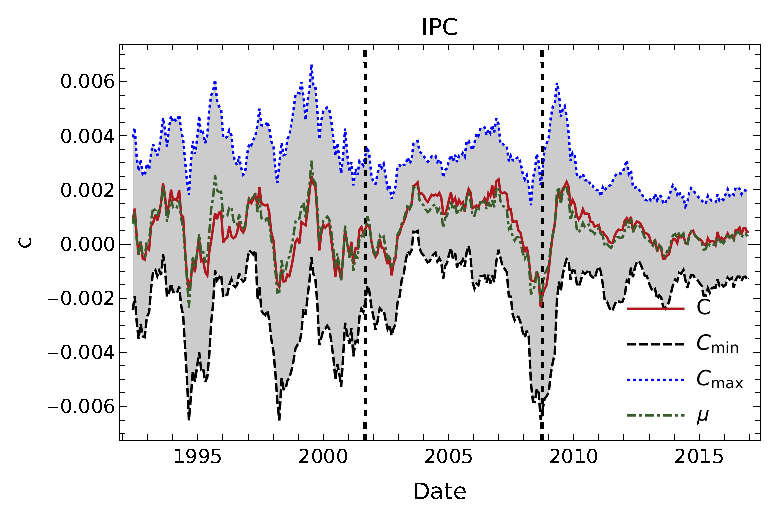
\includegraphics[scale=0.35]{img4/SimmReturns/Simetria_IPC_CL005}
		\end{subfigure}%
		\begin{subfigure}{.5\textwidth}
			\centering
			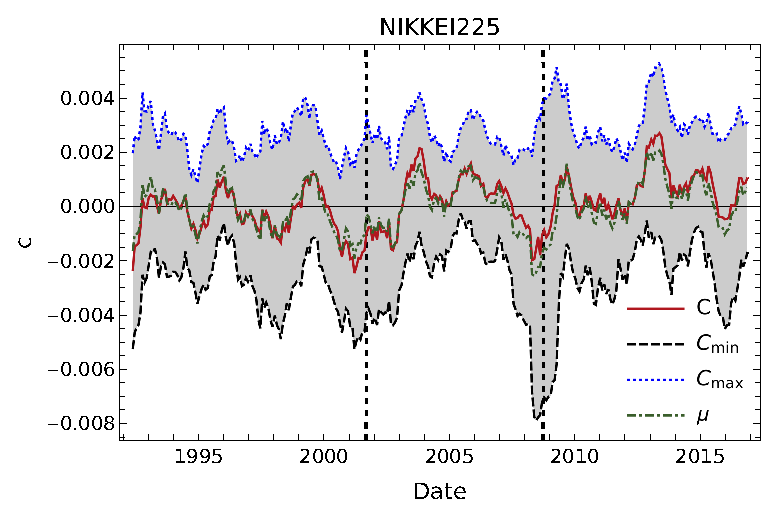
\includegraphics[scale=0.35]{img4/SimmReturns/Simetria_NIKKEI_CL005}
		\end{subfigure}%
	\end{figure}
\end{frame}

%-----------------------------------------------------------------------------
\begin{frame}
\frametitle{Time evolution of the most plausible point of symmetry: Trend returns}
  	  \begin{figure}[h!]
		\begin{subfigure}{.5\textwidth}
			\centering
			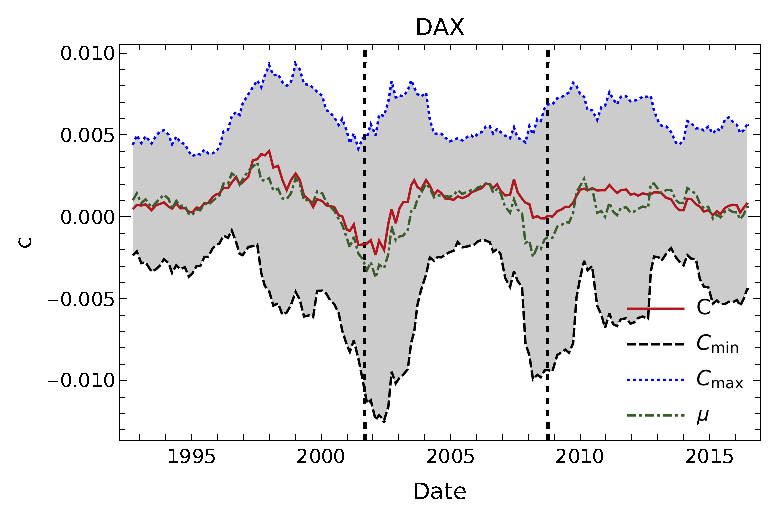
\includegraphics[scale=0.35]{img4/SimmTReturns/Simetria_DAX_CL005}
		\end{subfigure}%
		\begin{subfigure}{.5\textwidth}
			\centering
			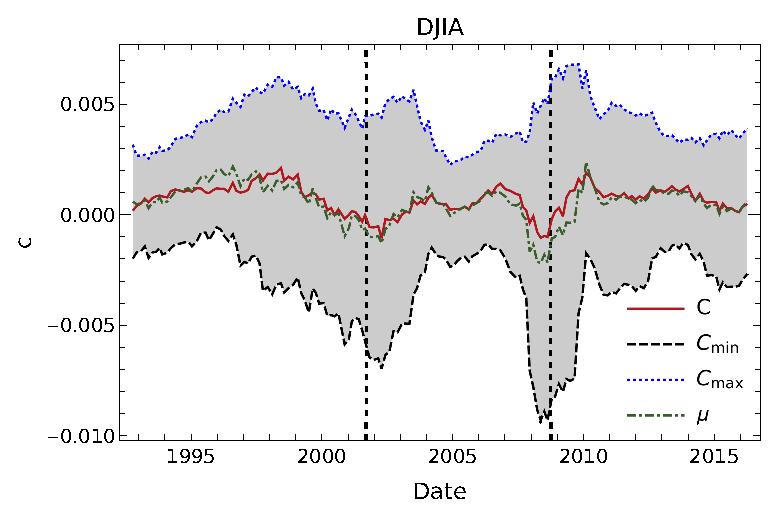
\includegraphics[scale=0.35]{img4/SimmTReturns/Simetria_DJIA_CL005}
		\end{subfigure}%
	\end{figure}
	  	  \begin{figure}[h!]
		\begin{subfigure}{.5\textwidth}
			\centering
			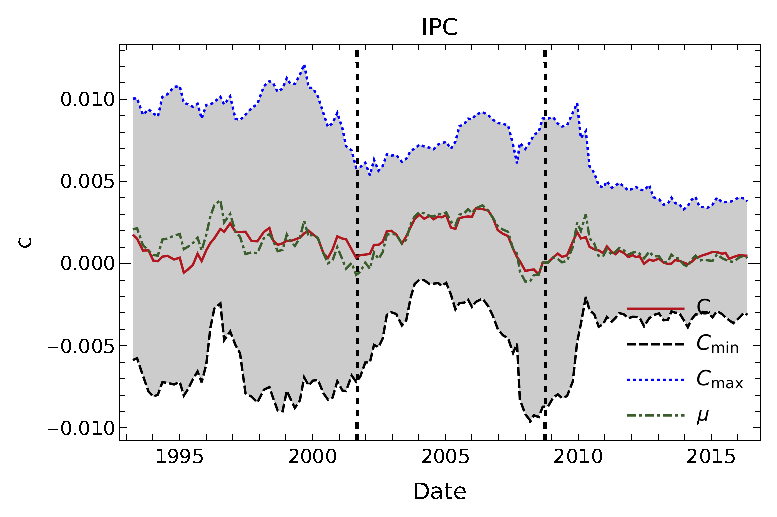
\includegraphics[scale=0.35]{img4/SimmTReturns/Simetria_IPC_CL005}
		\end{subfigure}%
		\begin{subfigure}{.5\textwidth}
			\centering
			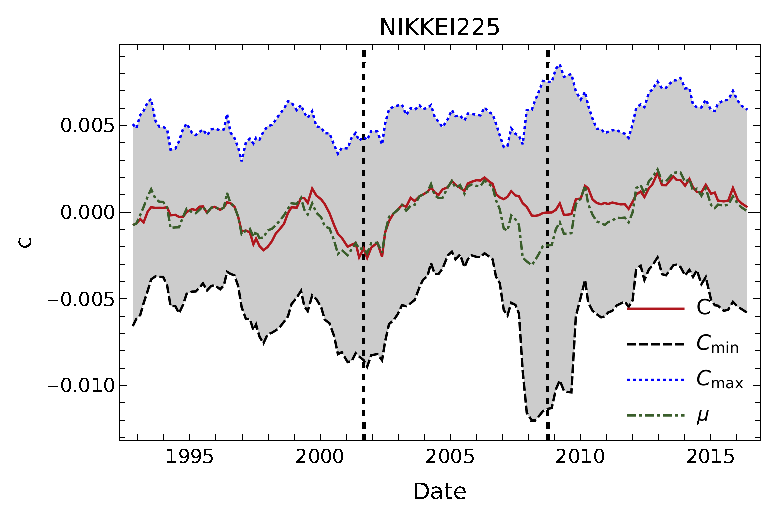
\includegraphics[scale=0.35]{img4/SimmTReturns/Simetria_NIKKEI_CL005}
		\end{subfigure}%
	\end{figure}
\end{frame}

%-----------------------------------------------------------------------------
\begin{frame}
\frametitle{Symmetry around zero}
  \begin{figure}
  	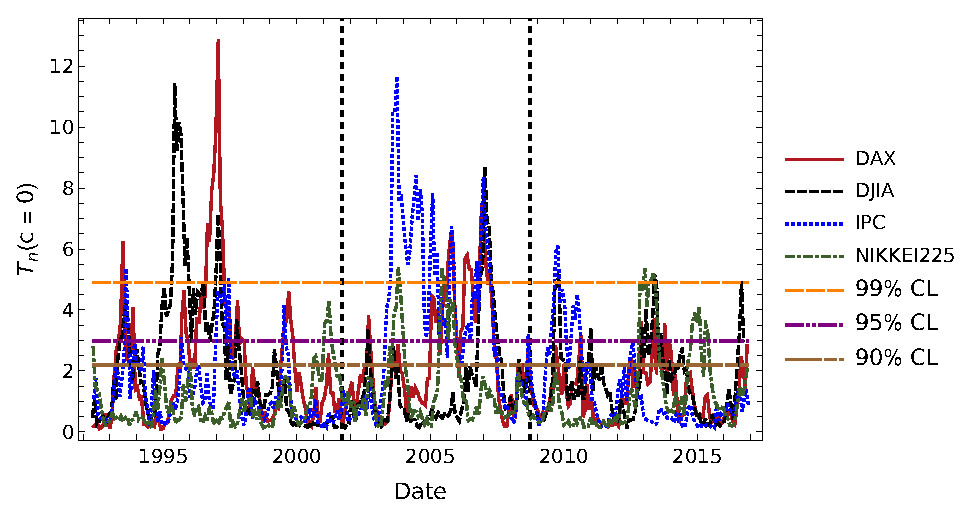
\includegraphics[scale=0.4]{img4/ZeroSymmetry/simetria_cero_tiempo_simpleret}
  \end{figure}
  \begin{figure}
  	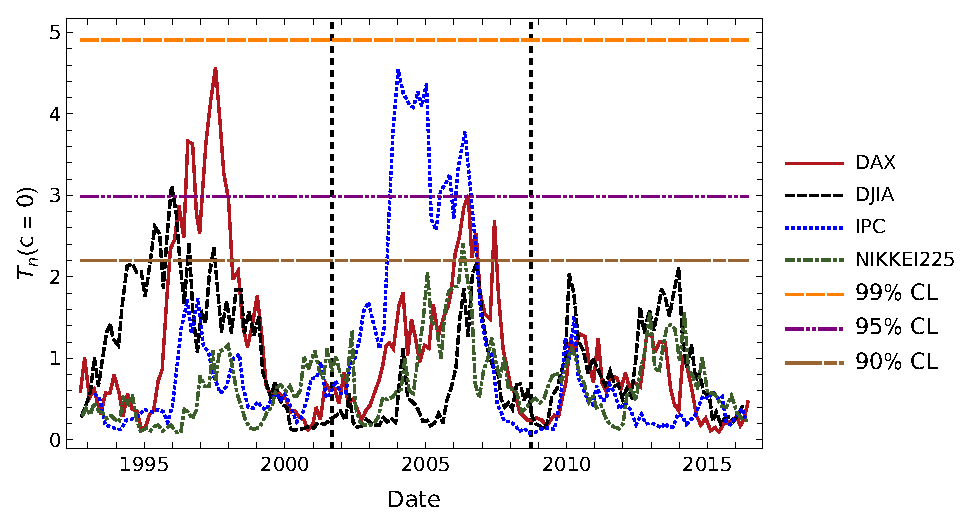
\includegraphics[scale=0.4]{img4/ZeroSymmetry/simetria_cero_tiempo_trendret}
  \end{figure}
\end{frame}

%-----------------------------------------------------------------------------
\begin{frame}
\frametitle{TRet and TVRet signals}
	The distributions of TRets and TVRets can be separated by run length by days.
  	  \begin{figure}[h!]
		\begin{subfigure}{.5\textwidth}
			\centering
			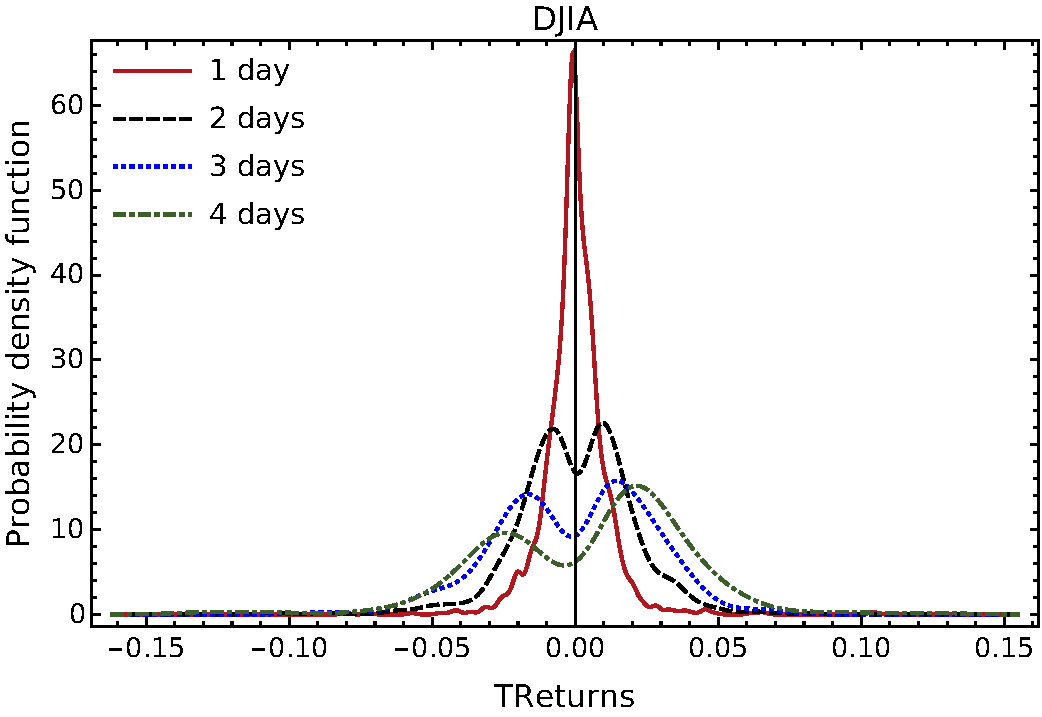
\includegraphics[scale=0.25]{img4/DecompositionByRun/dist_TRet_DJIA}
		\end{subfigure}%
		\begin{subfigure}{.5\textwidth}
			\centering
			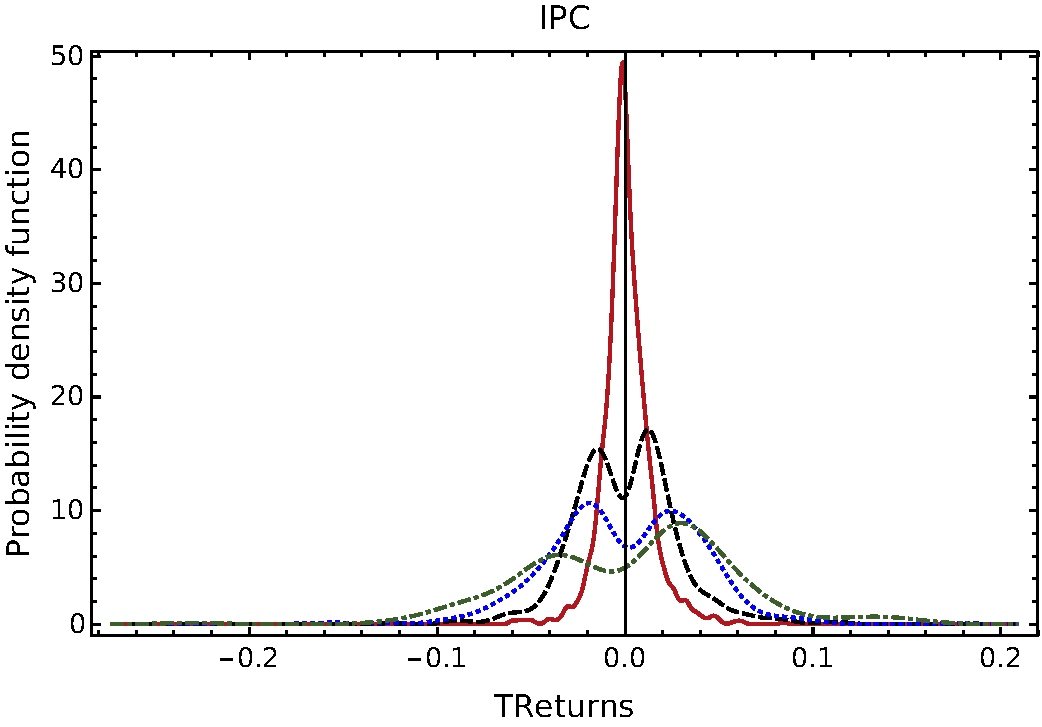
\includegraphics[scale=0.25]{img4/DecompositionByRun/dist_TRet_IPC}
		\end{subfigure}%
	\end{figure}
	  	  \begin{figure}[h!]
		\begin{subfigure}{.5\textwidth}
			\centering
			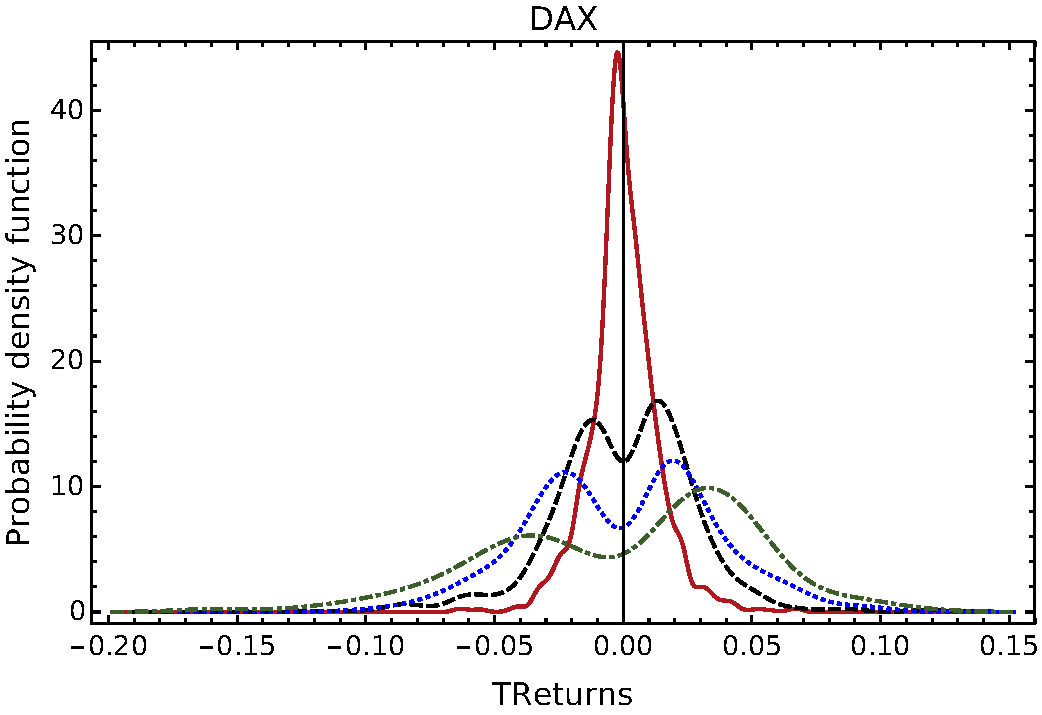
\includegraphics[scale=0.25]{img4/DecompositionByRun/dist_TRet_DAX}
		\end{subfigure}%
		\begin{subfigure}{.5\textwidth}
			\centering
			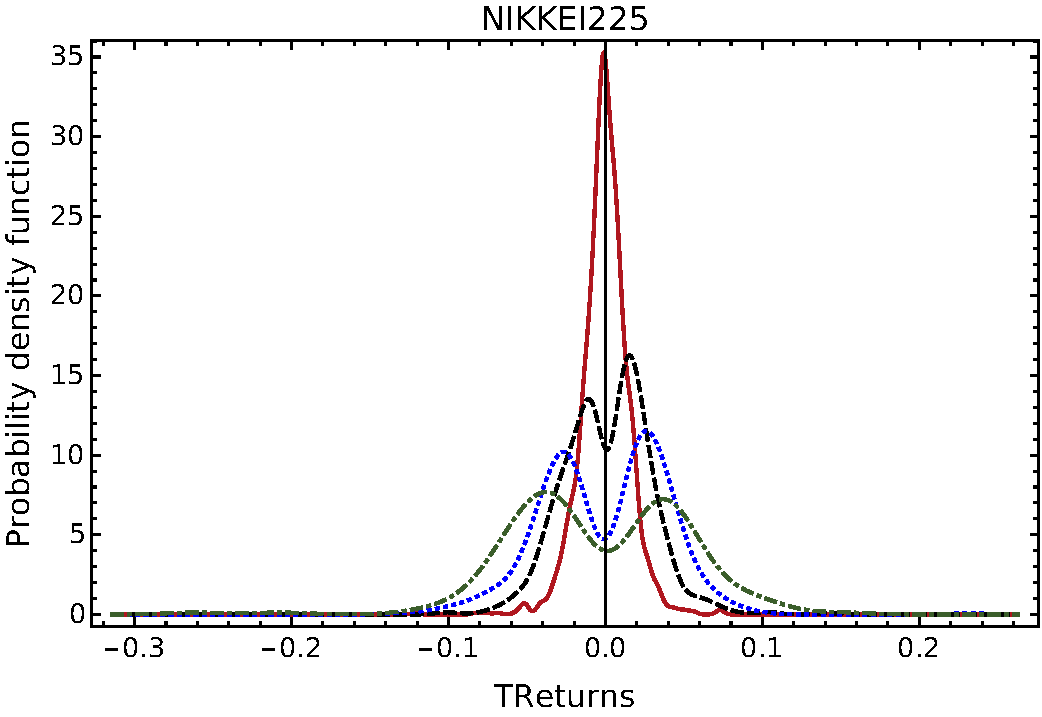
\includegraphics[scale=0.25]{img4/DecompositionByRun/dist_TRet_NIKKEI225}
		\end{subfigure}%
	\end{figure}
\end{frame}

%-----------------------------------------------------------------------------
\begin{frame}
\frametitle{TRet and TVRet signals}
	The shape of distributions of $k>1$ are more visible in TVRets because of the scaling done when dividing the TRets by run duration.
  	  \begin{figure}[h!]
		\begin{subfigure}{.5\textwidth}
			\centering
			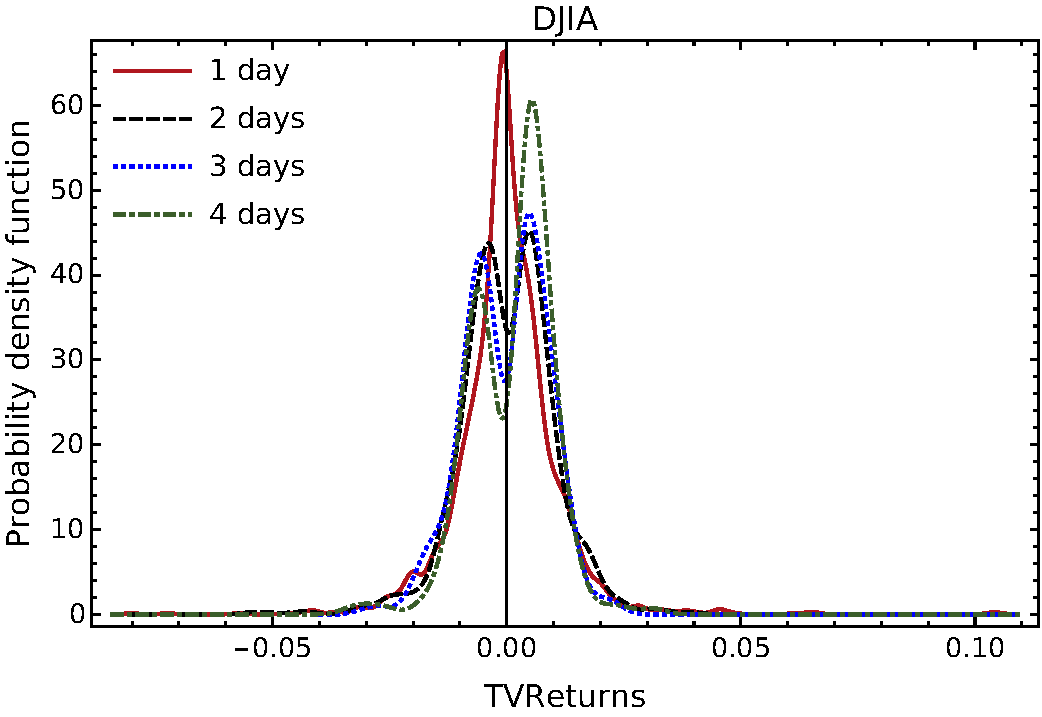
\includegraphics[scale=0.25]{img4/DecompositionByRun/dist_TVRet_DJIA}
		\end{subfigure}%
		\begin{subfigure}{.5\textwidth}
			\centering
			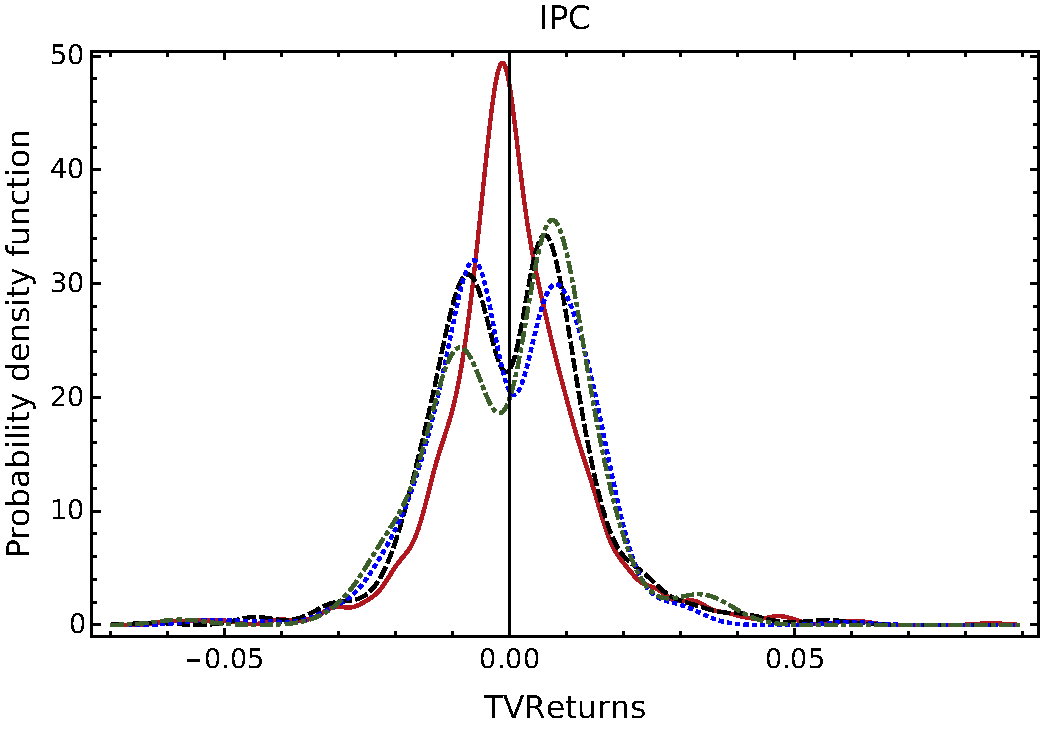
\includegraphics[scale=0.25]{img4/DecompositionByRun/dist_TVRet_IPC}
		\end{subfigure}%
	\end{figure}
	  	  \begin{figure}[h!]
		\begin{subfigure}{.5\textwidth}
			\centering
			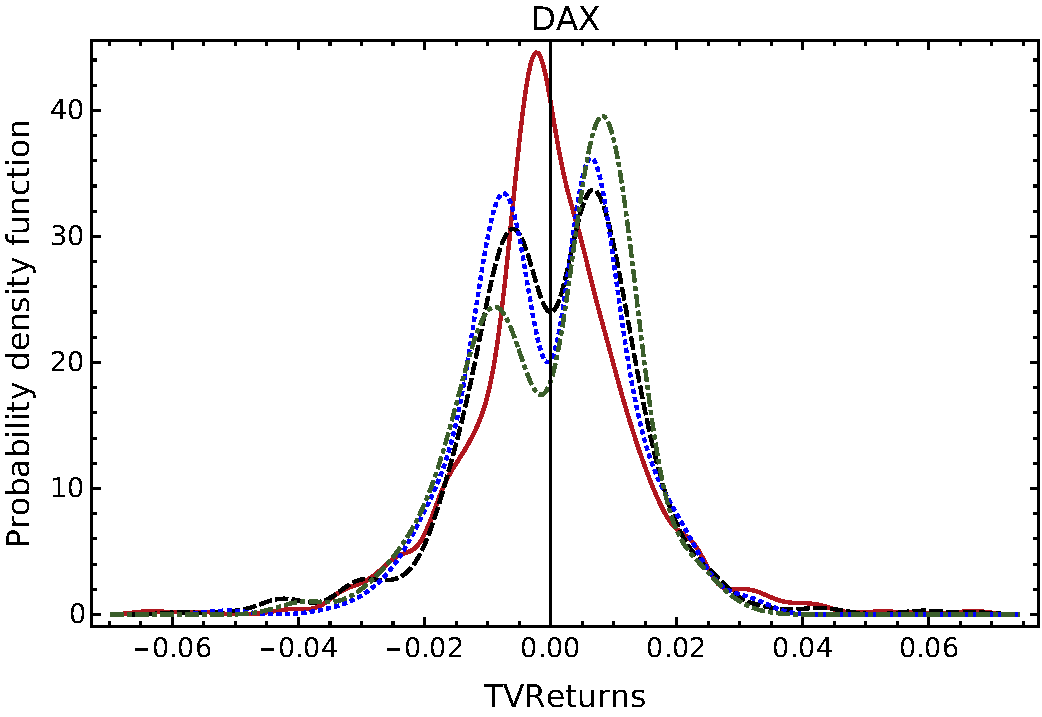
\includegraphics[scale=0.25]{img4/DecompositionByRun/dist_TVRet_DAX}
		\end{subfigure}%
		\begin{subfigure}{.5\textwidth}
			\centering
			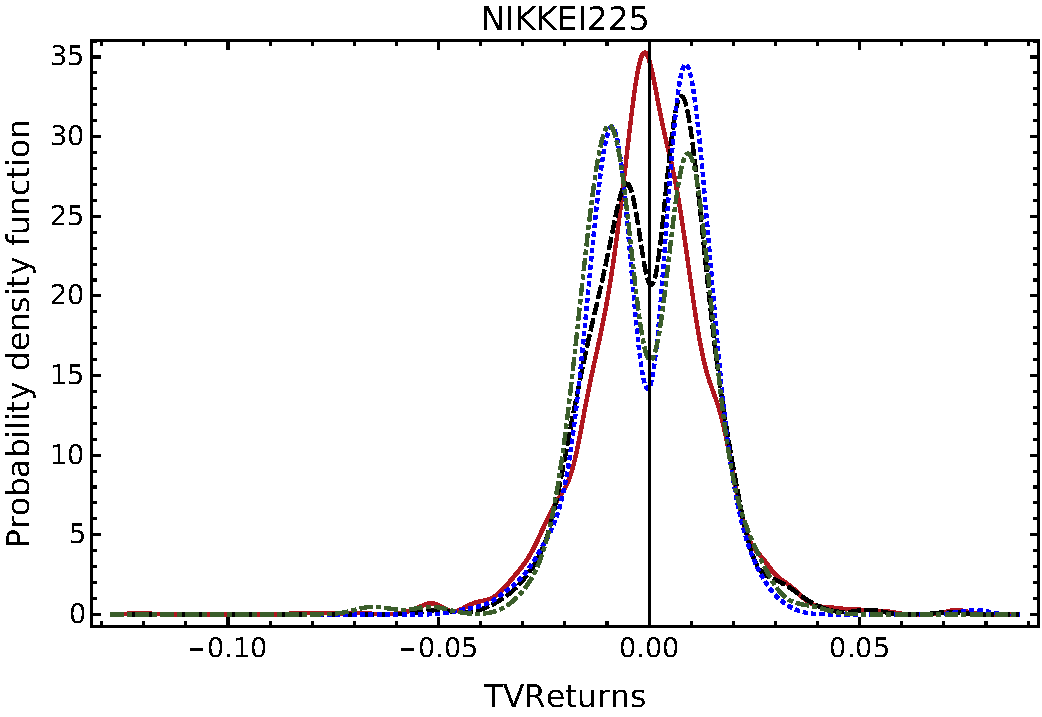
\includegraphics[scale=0.25]{img4/DecompositionByRun/dist_TVRet_NIKKEI225}
		\end{subfigure}%
	\end{figure}
\end{frame}


%-----------------------------------------------------------------------------
\begin{frame}
\frametitle{Conclusion}
  \begin{itemize}
  	\item We can measure symmetry of the returns using the $T_n$ statistic. We also defined the trend returns in order to select a scale independent observable.
  	\item Symmetry is not constant. Particularly symmetry around $c=0$ tends to be plausible in dates closer to extreme events.
  \end{itemize}
\end{frame}

%-----------------------------------------------------------------------------
\begin{frame}
Thank you all for your attention.
\end{frame}

\begin{frame}[noframenumbering,plain,allowframebreaks]
  \frametitle{Bibliography}
  \nocite{*}
  \printbibliography
\end{frame}

\end{document}